\documentclass[fontsize=11pt]{article}  
\usepackage{amsmath}  
\usepackage[utf8]{inputenc}  
\usepackage[margin=0.75in]{geometry}  
\usepackage[final]{graphicx}
\usepackage{subcaption}
  
\title{CSC111 Project Proposal: Interactive Music Genre and Album Recommendation Tree}  
\author{David Wu, Kevin Hu}  
\date{Tuesday, March 16, 2021}  
  
\begin{document}  
\maketitle  
  
\section*{Problem Description and Project Goal}  
  
To many of us, music is a large part of our lives, helping us get through the day. According to the International Federation of the Phonographic Industry (IFPI), the average person spent 18.4 hours a week listening to music in 2021\textsuperscript{1}. With the sheer number of music available on modern streaming platforms such as Spotify or Apple Music, it can be extremely difficult and time-consuming for the casual listener to find new music that they enjoy, especially since listeners themselves may not know what they like. A listener may know that they typically enjoy Rock music but "Rock" is a broad term that encompasses many distinct subgenres, perhaps they are into the raw, distorted sound of Noise Rock or maybe they prefer the more technical, complicated time signatures of Math Rock. This is not to mention that different albums within a subgenre could also be further categorized by different descriptors such as warm, aggressive or depressing. The casual listener is simply unaware of these distinctions when trying to find something they like on the Rock section of Spotify. We believe that good music recommendations should be fast and easy. \textbf{Our goal is to provide users with the best possible song recommendations, given the current preferences of the user in either the form of a preferred genre or a favourite album,} letting users spend less time looking for music and more time listening. This would be done with a visual element in the form of a tree, with the best recommendations located towards the top, and the subsequent branches giving the user options to discover other musical pathways on their own. We would also provide an interactive element for users to further explore their recommendations and how they fit within the larger tree of music genres and albums, allowing users to potentially discover new songs and albums they can enjoy, without having to search through individual songs on music streaming sites.  
  

  
\section*{Datasets Used}

~~~1. Rate Your Music: The Top 5,000 Most Popular Albums(rym\_clean1.csv)\textsuperscript{2} \newline

Found on kaggle, this dataset contains 5,000 of the most popular albums found on the music database and review website rateyourmusic.com (RYM). The popularity of the albums was determined by the number of reviews each album had, showing the number of meaningful interactions. As a downloadable csv file with the name \texttt{rym\_clean1.csv}, each line contains the information of a specific album, with the following attributes in order: \texttt{position}(popularity rank), \texttt{release\_name}, \texttt{artist\_name}, \texttt{release\_date}, \texttt{release\_type}, \texttt{primary\_genres}, \texttt{secondary\_genres}, \texttt{descriptors}, \texttt{avg\_rating}, \texttt{rating\_count}, and \texttt{review\_count}. In our program, we will primarily use the \texttt{position}, \texttt{release\_name}, \texttt{artist\_name}, \texttt{primary\_genres}, \texttt{release\_date}, and \texttt{descriptors} attributes for computations. Our program also utilizes all 5001 lines in the csv file to generate the best possible recommendations(excluding line 1 with includes the header information). \newline

~~~2. Genres Dataset(genres\_dataset.csv) \newline

Using information from rateyourmusic.com (RYM)\textsuperscript{3}, we generated a data set containing all music genres and subsequent subgenres found on RYM. In the file \texttt{genres\_dataset.csv}, each line contains the information of a music genre, with the attributes in the order \texttt{genre}, \texttt{parent genre}. \texttt{genre} is the name of the genre, while \texttt{parent genre} is the genre under which Genre may be listed. If \texttt{genre} is a main genre with no parent genre, \texttt{parent genre} is given the value \texttt{NA}. All attributes are used for computations in our program, as well as all 1817 lines in the csv while(excluding line 1 with includes the header information). \newline

\section*{Computational Overview} 
As the main database for our recommendations(\texttt{rym\_clean1.csv}), we will use the top 5,000 most popular albums pulled from the music review site rateyourmusic.com (RYM). As mentioned in the previous section, the main attributes we will be utilizing are \texttt{position}, \texttt{release\_name}, \texttt{artist\_name}, \texttt{primary\_genres}, \texttt{release\_date}, and \texttt{descriptors} to help with recommendation computations and visualizations. To help identify genres and their subgenres, we have created a genres dataset(\texttt{genres\_dataset.csv}), which contains the name of all music genres listed on RYM, and their parent genre if there are any. Our projects will then primarily use trees to represent the genres and albums in our datasets in a hierarchical manner, with three main trees: the genre tree, the genre recommendation tree, and the album recommendation tree. Starting with the genre tree, this tree is separate from the other recommendation tree as it serves as more of an informational role. The starting node of the tree just has the title "Genre", which branches off into the main music genres(i.e. the genres with no parent genre), and then the tree branches off into the subgenres. As for the album recommendation tree, its root will be an album inputted by the user(the album will be from the top 5,000 albums dataset). From there, the tree will branch into the top recommendations, which will be calculated by finding other albums in the dataset with the most matching strings from the descriptors attribute. The tree will then recurse through the top recommendations as if they were the album inputted in by the user, but will also avoid using already recommended albums for further subtrees. The genre recommendation tree is similar to the album recommendation tree, except the root will instead be a genre inputted by the user. The first group of subtrees will then be the most popular albums of the inputted genres. From there, further subtrees will be added using the same recommendation algorithm used in the album recommendation tree. \newline 

To extract data from our datasets, we have created the \texttt{genres\_data} and \texttt{albums\_data} files, which contain the \texttt{Genre} class and \texttt{Album} class respectively. These classes serve to represent each individual genre and album, with the relevant attribute pulled from the top 5,000 most popular albums dataset, and genres dataset. Here is a look at the Album class:
\begin{verbatim}  
    class Album:  
    """  
    a class to represent an album.  
    """  
    name: str  
    artist: str    
    genres: list[str]  
    rank: int  
    release: str  
    descriptors: list[str]  
\end{verbatim}  
The instance attributes include the name of the album, the name of the artist, a list of the album's associated genres, its position on the music database RateYourMusic's list of most popular albums, it's the release date and a list of descriptors for the album. Using an import from \texttt{csv}, the \texttt{albums\_data} file will also read the data from the top 5,000 most popular albums dataset, converting each line in the dataset into an \texttt{Album} object, and storing everything from this dataset into a list called \texttt{albums}, which is a list of \texttt{Album} instances. This \texttt{albums} list will later be imported into other classes and files for computations. The \texttt{genre\_data} file is similar to \texttt{albums\_data}, except it only has the instance attributes \texttt{name}(a string), and \texttt{parent\_genre}(which is defined as \texttt{Optional[str]}). \texttt{parent\_genre} is \texttt{None} when the genre is a main genre. Using \texttt{csv} imports again, each line in the genres dataset is read and converted into a \texttt{Genre} instance, which is all saved into a list called \texttt{genres}. \newline

The main tree structures and methods are provided in \texttt{tree\_classes}. Within the \texttt{tree\_classes} file contains the class \texttt{Tree}, with the typical implementation and instance attributes \texttt{\_root}(which is defined as \texttt{Optional[Any]}) and \texttt{\_subtrees}(which is defined as \texttt{list[Any]}). \texttt{Tree} is also implemented with some of the standard methods(i.e. \texttt{is\_empty}). The child class \texttt{Album Tree} is also implemented here, which is initialized the same way as \texttt{Tree}. \newline

The major computations of our program are done in the \texttt{plot\_recommendation\_tree} and \texttt{plot\_genre\_tree} files. Examining \texttt{plot\_recommendation\_tree}, the main attraction of our program, the recommendation algorithm is done through the function \texttt{get\_albums\_by\_matches}, which outputs a list of  \texttt{Album} instances. Taking in a given \texttt{Album} and a list of \texttt{Album} instances, this function compares the number of matching \texttt{descriptors} from the given \texttt{Album} and each album in the list of \texttt{Album} instances(as long as the given \texttt{Album} is not the same as the compared \texttt{Album}). This function also takes in a visited set, stopping comparisons from the given \texttt{Album} to any albums in \texttt{visited}, which is later used for tree generation. After each comparison between the given and compared to \texttt{Album}, the compared to \texttt{Album} is stored in a dictionary \texttt{album\_to\_matches}, mapping the \texttt{Album} name to the actual \texttt{Album} instance, and the number of matches. The final parameter of this function is \texttt{num\_recommendations}, which is an \texttt{int} that decides how long the output list is. Based of \texttt{num\_recommendations}, that number of albums is pulled out of \texttt{album\_to\_matches} with the highest number of matches for \texttt{descriptors} being pulled first. This also results in the output to \texttt{get\_albums\_by\_matches} being a sorted list, with the earlier elements having more matches than the later elements. The next main function is \texttt{generate\_album\_recommendation\_tree}, which is what actually creates the frame for the album recommendation tree. It takes in a \texttt{depth} parameter to control the size of the tree. Then, from a given \texttt{root\_album}, the function uses the algorithm from \texttt{get\_albums\_by\_matches} to find the best-recommended albums and creates a subtree for each recommendation. \texttt{generate\_album\_recommendation\_tree} then recuses through each subtree to further develop the recommendation tree. A visited set is taken in by this function, which is fed into \texttt{get\_albums\_by\_matches} to make sure further subtrees down the tree don't repeat the same recommendations. The actual visualization of the album recommendation tree is then done through the function \texttt{plot\_album\_recommendation\_tree}, which further explores the \texttt{plotly} library and the \texttt{igraph} library. Using the implementation  of tree plots found in the \texttt{plotly} library\textsuperscript{5}, \texttt{plot\_album\_recommendation\_tree} generates a visualization of the tree generated from \texttt{generate\_album\_recommendation\_tree}, using the roots and branches of the tree(i.e. vertices and edges). To get all the vertices and edges of a tree, two recursive helper functions, \texttt{get\_all\_branches} and \texttt{get\_all\_vertices} was created. Both have essentially the same implementation, recursing through a given tree and saving all vertices or edges(a tuple of vertices) into a list. Using the list of vertices and edges obtained from these helper functions, \texttt{plot\_album\_recommendation\_tree} creates a visualization of the tree. \newline

\begin{figure}[h]
    \centering
    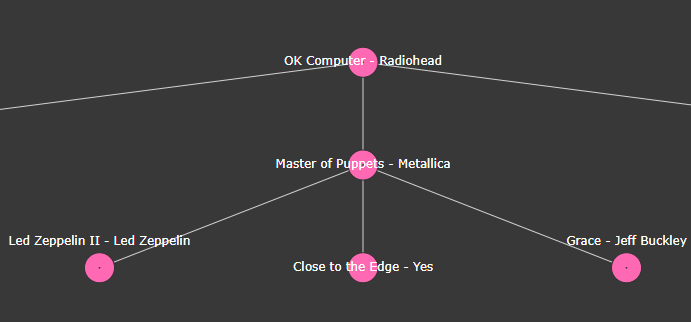
\includegraphics[height=7cm, width=13cm]{exampletree.png}
    \caption{Example plot of the album recommendation tree}
    \label{fig:my_label}
\end{figure}

As for the genre recommendation tree, when the user inputs a genre, the top albums of the inputted genre are outputted, and then the album recommendation tree takes over for further subtrees. Only the root and direct subtrees are needed for the genre recommendation tree, so there is no need to create a separate tree generation function. Instead, given the \texttt{name} attribute of a \texttt{Genre}, the function \texttt{get\_albums\_by\_genre\_and\_popularity} takes in a list of \texttt{Album} instances and filters it, returning a list of \texttt{Album} instances with the same genre name as the inputted \texttt{Genre}. This function was also intended to sort the returned list of \texttt{Album} instances from most to least popular, however, due to the top 5,000 albums dataset already being sorted in order by popularity, the inputted \texttt{albums} list is already sorted, so \texttt{get\_albums\_by\_genre\_and\_popularity} only acts as a filter. \texttt{get\_albums\_by\_genre\_and\_popularity} is then used in \texttt{plot\_genre\_recommendation\_tree} to find recommendations for a given genre. \texttt{plot\_genre\_recommendation\_tree} has the same \texttt{plotly} implementation as \texttt{plot\_album\_recommendation\_tree}, with the edges instead being between the inputted \texttt{Genre} and the outputs from \texttt{get\_albums\_by\_genre\_and\_popularity}. \texttt{plot\_genre\_recommendation\_tree} will then display a tree with at most 10 recommendations for the inputted. \newline

In the file \texttt{plot\_genre\_tree}, this is used to create a visualization for the informational genre tree, but still uses the same \texttt{plotly} implementation as \texttt{plot\_album\_recommendation\_tree} and \texttt{plot\_genre\_recommendation\_tree} for tree plot visualizations. Using the list of genre names \texttt{genres} from \texttt{genres\_data} the \texttt{name} attribute of each \texttt{Genre} in the list is made into a vertex, and an edge from each \texttt{Genre}'s \texttt{name} attribute to its \texttt{parent\_genre} is created. These vertices and edges are used in both plotting functions in \texttt{plot\_genre\_tree}.

\section*{Instructions for Use}

First, install the libraries listed in the \texttt{requirements.txt} file. The two dataset for our program, \texttt{rym\_clean1.csv} and \texttt{genres\_dataset.csv} can be found on MarkUs, in a zip folder labelled \texttt{datasets}. After downloading the required files from MarkUs as well, run the file \texttt{main.py}. In the console, a link developed through Plotly Dash should appear(after the text 'Dash is running on'). Click the link to open the program.

Once the program is launched, it should look something like this: 

\begin{figure}[h]
    \centering
    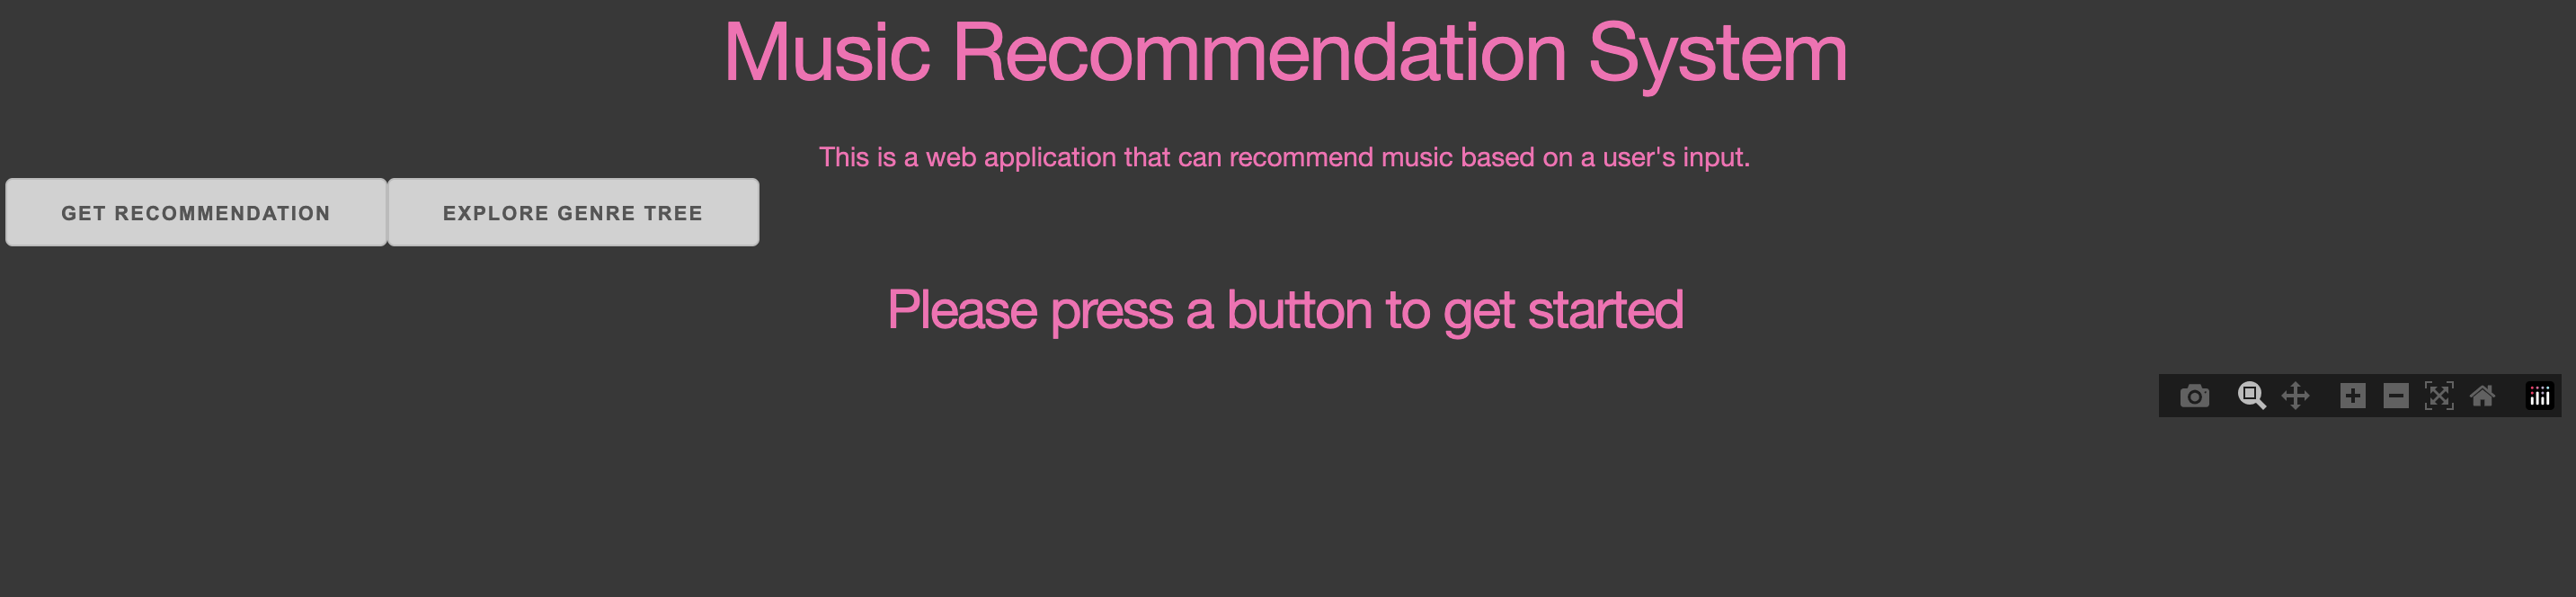
\includegraphics[height=7cm, width=18cm]{examplelaunch.png}
    \caption{Initail display upon opening the program}
    \label{fig:my_label}
\end{figure}

There are two buttons towards the top left, labelled 'GET RECOMMENDATION' and 'EXPLORE GENRE TREE'. Clicking 'EXPLORE GENRE TREE' will display the genre tree. Clicking on each of the nodes of the subtrees will allow you to further explore down the subgenres of the node clicked. There is also a go-back button on the left to go back to the previous tree before the node was clicked. 

\begin{figure}[h]
    \centering
    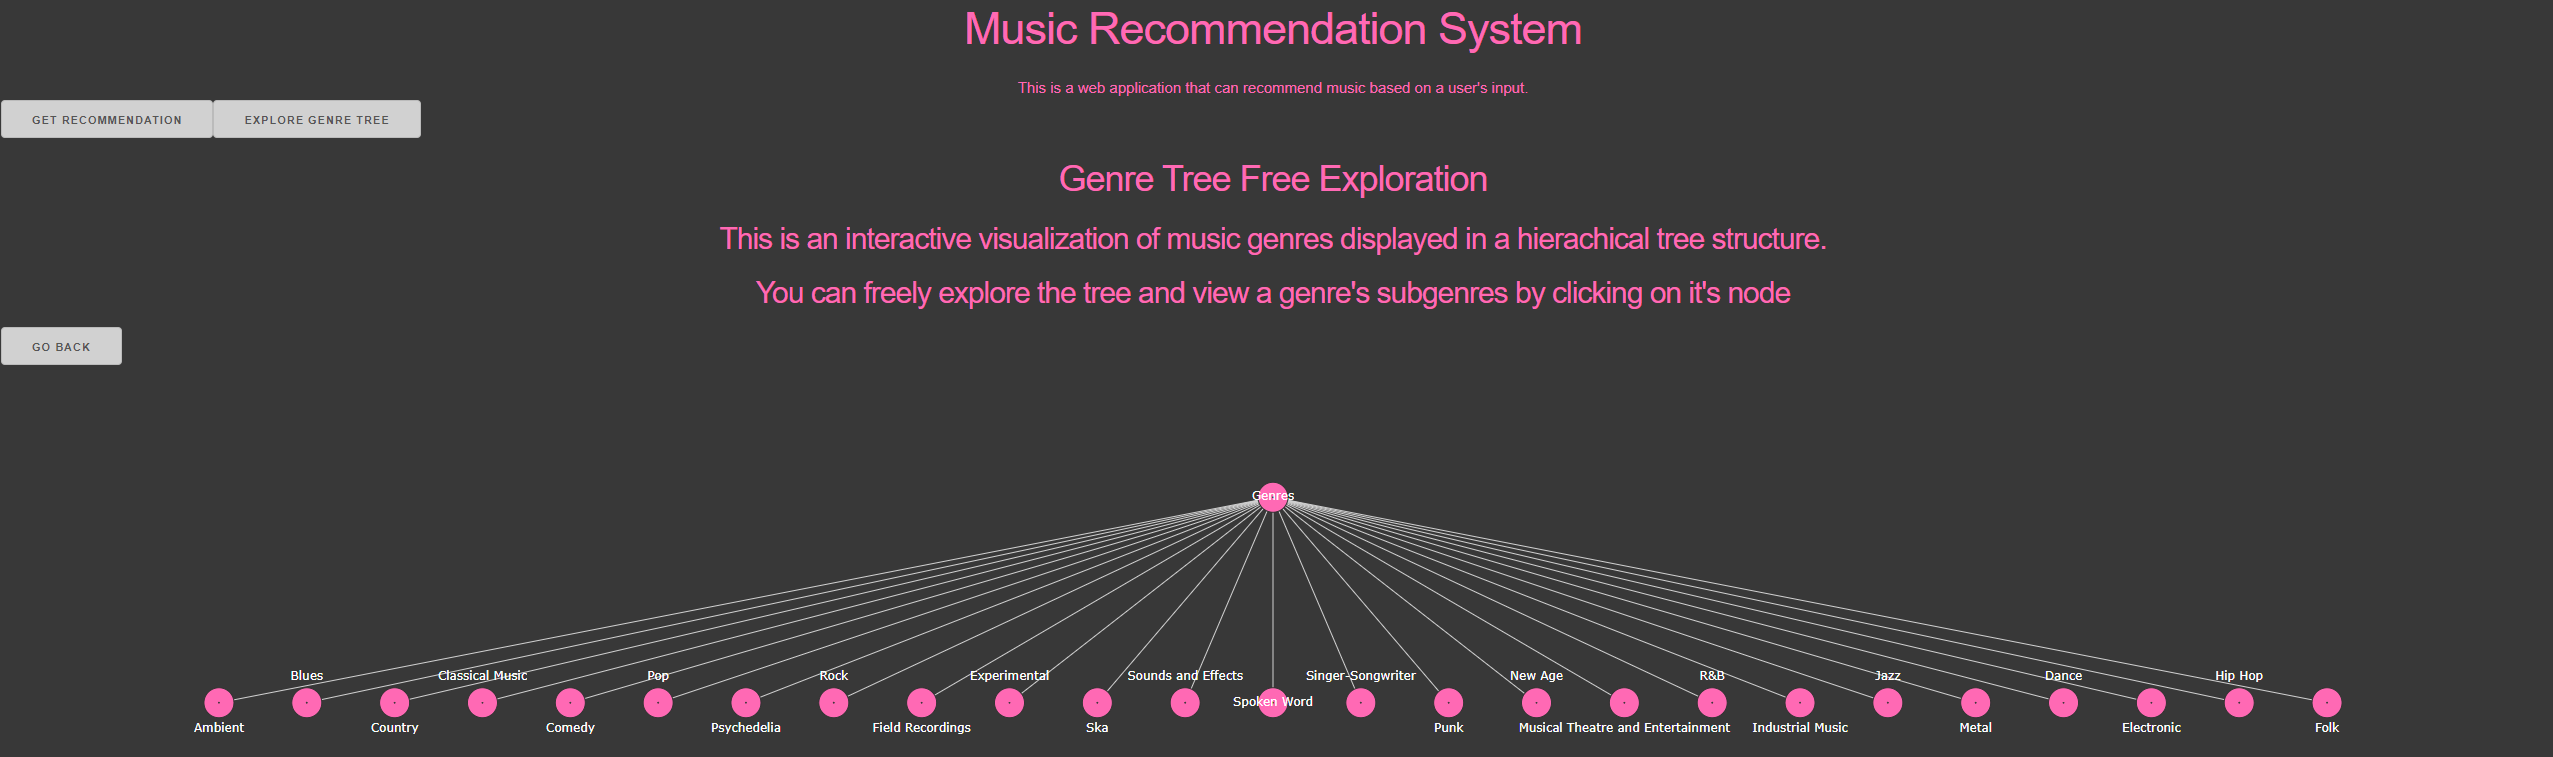
\includegraphics[height=7cm, width=18cm]{examplegenretree.png}
    \caption{Display when exploring genre tree}
    \label{fig:my_label}
\end{figure}

For the button 'GET RECOMMENDATION', two search bars pop up. The top search bar is used when inputting a preferred album(album recommendation tree). If an album is inputted into the top search bar, click the 'SUBMIT ALBUM' button below to generate a recommendation tree base on the inputted album. Similar to the genre tree, the nodes of this tree(which are albums) can be clicked to further explore the recommendations from the clicked-on album. The bottom search bar is used for inputting genres for the genre recommendation tree. If a genre is inputted into the bottom search bar, click the 'SUBMIT GENRE' button to generate a genre recommendation tree for the respective input. The nodes of this tree(albums) can also be clicked through to further explore each musical pathway.

\begin{figure}[h]
    \centering
    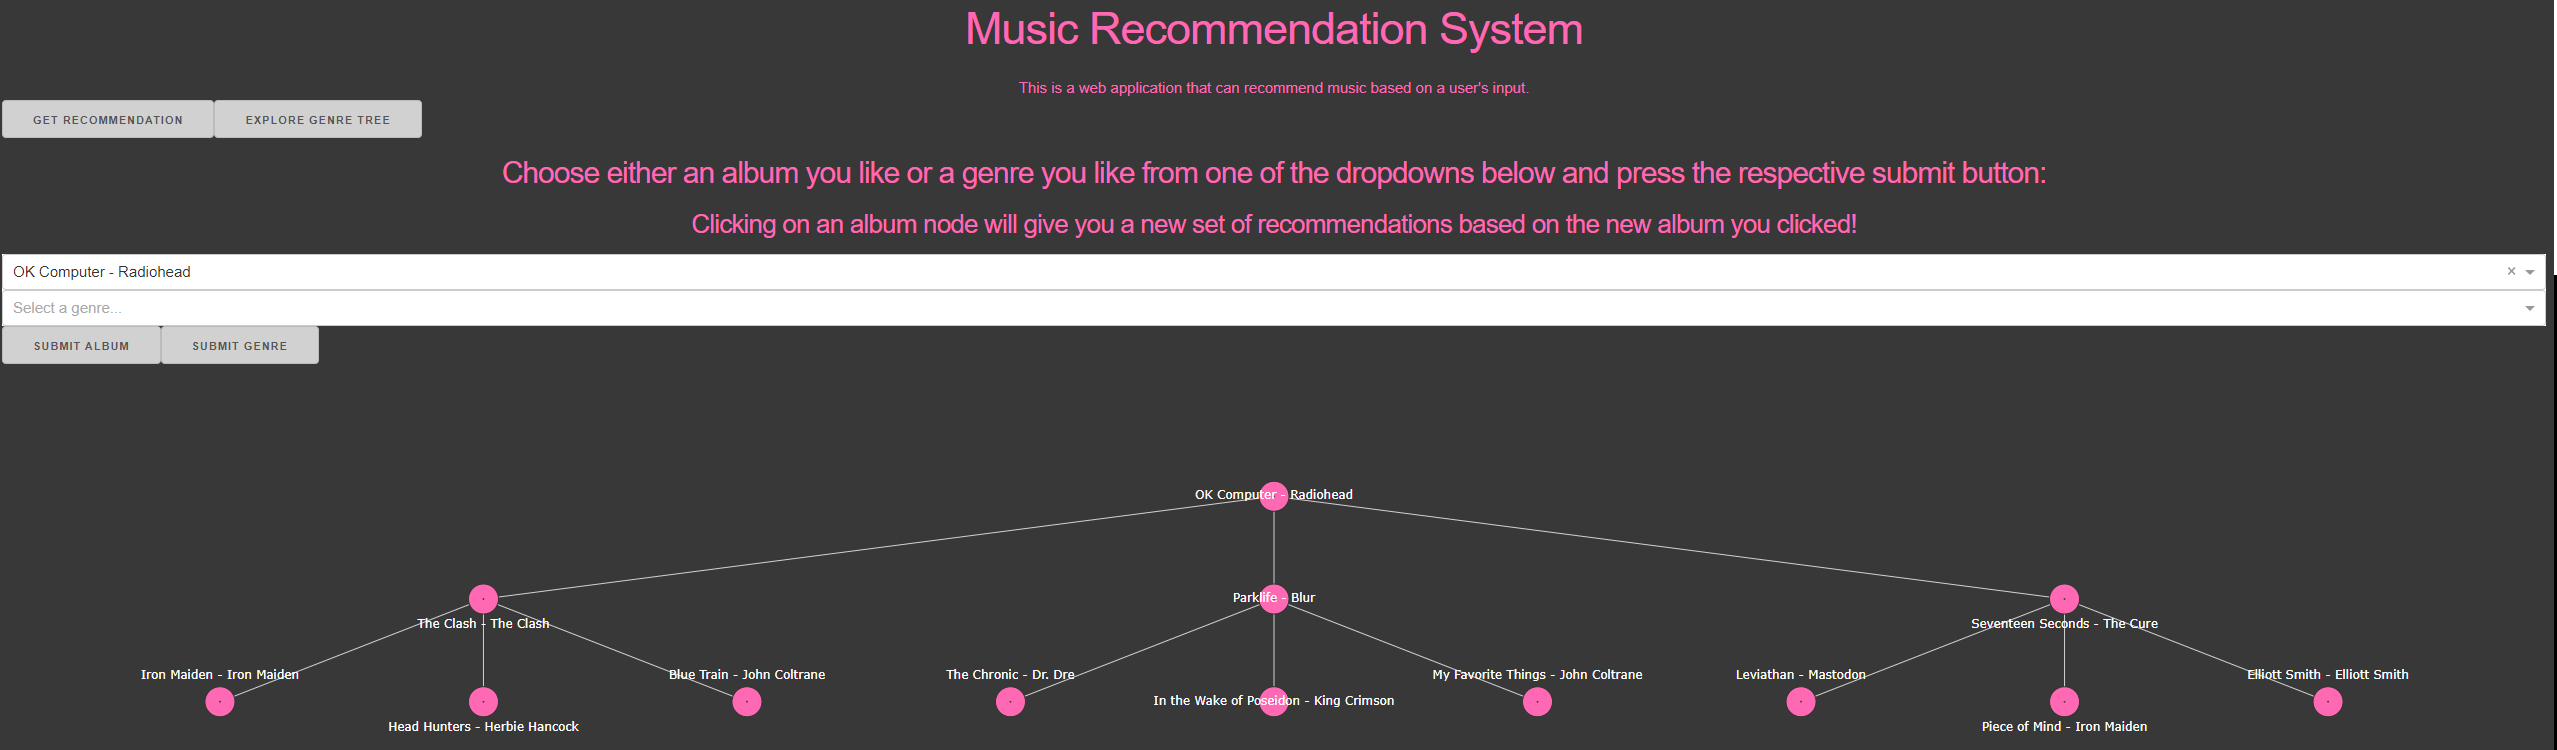
\includegraphics[height=7cm, width=18cm]{examplerun.png}
    \caption{Display when using the recommendation trees}
    \label{fig:my_label}
\end{figure}

\section*{Changes to Project Plan}

From our original project proposal, overall, we have not changed much. Our original project goal has stayed as same(as outlined in the Problem Description and Project Goal section), and we have created our three genre trees, genre recommendation tree, and album recommendation tree as intended. As cited in our original project proposal, we have also continued on using Plotly tree plots\textsuperscript{5} and Plotly Dash\textsuperscript{4} to create a visualization of our created trees, and an interactable interface for the user. After given some suggestions, we considered using the Tkinter library(notably Tkinter \texttt{treeview} and Tkinter \texttt{pytree}, however after some struggles to create a clean interface to display both the graph and interactable elements, we decided to continue with Plotly. As for the mention of using the Spotify API in our project proposal to give a playback of the recommended album, we decide to use Spotipy to implement this feature. 

\section*{Analysis and Interpretation of Results}

Overall, we have achieved our goal of providing a convenient way to get song recommendations given a preferred genre or album. Through a couple of clicks, users can easily see the recommendations for their input in a hierarchical manner, with better recommendations intuitively found at the top near the input. Users can also explore new songs and genres by simply clicking on a recommendation they like. Due to the use of trees and their recursive implementation, users can potentially explore a continuous branch of subtrees with albums they enjoy. If they like a certain recommendation, they can go further down into the subtrees of that recommendation. We believe our use of album descriptors in our recommendation algorithm also is better than simply using genres, which is why the main feature of our program is the album recommendation tree. While people often have a preferred genre, only recommending albums of a specific genre may be too limiting, and doesn't allow the user to potentially explore new albums and genres they may actually like. From our vision developed during our project proposal, we are satisfied with the result \newline

However, while we have provided a quick and convenient way to find song recommendations, whether these are the 'best' recommendations is up for debate. First is the limitation of our datasets, which only contains 5,000 albums, found as the most popular albums on rateyourmusic.com (RYM). There are likely millions of music albums in the world, but our recommendation tree only builds off the information from RYM. This dataset also is of the most popular albums, not individual songs. A user may only like one or two songs from a certain album, possibly wasting time for them. Our genre dataset, it is also limited to the genres on RYM, which may be labelled/described differently from other sources. Due to the limited scope of the datasets, our recommendation trees are building off of, it is hard to tell how well it produced good recommendations. Another limitation is in combination with our recommendation algorithm and datasets. While we believe album descriptors are an overall better measure for recommendations than genres, the algorithm is still limited to one element of the album. These descriptions are also once again, limited to the descriptors found on RYM. It may be difficult to produce good recommendations when only one attribute of the albums is considered. \newline

For future exploration, updating the recommendation algorithm to use multiple parameters, such as adding the genre, release date, artist, and more may help produce better recommendations. Adding more datasets to allow the algorithm to use more songs and albums would also be beneficial, though the running time of the program may increase. We were also given the suggestion to implement the recommendation trees as binary search trees(BSTs), with albums that have more matches located on the right, and albums with fewer matches on the left. While this implementation isn't necessarily a better way to organize recommendations, it does provide a different viewpoint, which may be preferred to be some users. An option to switch between the current implementation and the BST implementation can be another future idea to improve the accuracy of recommendations. \newline

To reiterate our goal, we wanted to provide users with the best possible song recommendations knowing their current preferences for a certain music genre or album. Using implementations with trees, we first provided an informational genre tree was also provided to help guide users through the different music genres, helping them discover any new genres they may like. The recommendation trees were then constructed with the most popular albums or albums with the most matching descriptors located toward the top, and the recursive nature of the tree allowed users to further explore a line of albums they liked. However, due to limitations in the size of our datasets and the linearity of our sorting algorithm, possible album recommendations may not be the best. For better recommendations, adding more data from a variety of sources, as well as incorporating more parameters to the sorting algorithm can help improve recommendations. While this program may not be perfect, we were able to provide quick and relevant song recommendations with an intuitive visualization to help users get a start on their musical journey.

\section*{References}  
~~~~1. IFPI. (2021). Engaging with Music. https://www.ifpi.org/wp-content/uploads/2021/10/IFPI-Engaging-with-Music-report.pdf \newline  
  
2. Bryan O. (2022, March). Rate Your Music: The Top 5,000 Most Popular Albums, Version 1, Retrieved March 8, 2023 from https://www.kaggle.com/datasets/tobennao/rym-top-5000 \newline  

3. Sonemic (n.d.). RateYourMusic All Music Genres. https://rateyourmusic.com/genres/  \newline 

4. Plotly Dash. (n.d.). Introduction | Dash for Python Documentation. https://dash.plotly.com/introduction \newline  
  
5. Plotly (n.d.). Tree Plots in Python. https://plotly.com/python/tree-plots/ \newline  
‌  
6‌. Richardson, L. (2007). Beautiful soup documentation. https://www.crummy.com/software/BeautifulSoup/bs4/doc/ \newline  
  
7. Reitz, K. (n.d.). Requests: HTTP for Humans™. https://requests.readthedocs.io/en/latest/ \newline  
  
8. Spotify (n.d.). Spotify Web API. https://developer.spotify.com/documentation/web-api/reference/\#/ \newline  
  
% NOTE: LaTeX does have a built-in way of generating references automatically,  
% but it's a bit tricky to use so we STRONGLY recommend writing your references  
% manually, using a standard academic format like APA or MLA.  
% (E.g., https://owl.purdue.edu/owl/research_and_citation/apa_style/apa_formatting_and_style_guide/general_format.html)  
  
\end{document}  
